\documentclass[aspectratio=169]{beamer}
\usetheme{Darmstadt}

\usepackage{amsmath, amssymb}
\usepackage{algorithm,algorithmicx,algpseudocode}
\usepackage{tikz}
\usetikzlibrary{matrix,decorations.pathmorphing,calc,decorations.pathreplacing,topaths,fit,positioning,automata,patterns,arrows,shapes,chains}
\tikzstyle{line} = [draw, -latex']

% Commands
\newcommand{\dd}{\,\text{d}}
\newcommand{\T}{\text{T}}
\newcommand{\B}[1]{\mathbf{#1}} % shortcut for \mathbf
\newcommand{\Bs}[1]{\boldsymbol{#1}} % shortcut for \boldsymbol
\newcommand{\pr}[1]{\left(#1\right)} % shortcut for \left(\right)
\newcommand{\br}[1]{\left[#1\right]} % shortcut for \left[\right]
\newcommand{\bbr}[1]{\left\{#1\right\}} % shortcut for \left\{\right\}
\newcommand{\nr}[1]{\left\|#1\right\|} % shortcut for \left\|\right\|

\title{High-Dimensional Gaussian Sampling}
\author{Yuejia Zhang}
\date{April 7, 2023}
\begin{document}
	
\begin{frame}
    \maketitle
\end{frame}

\section{Introduction} 
\subsection{Problem}
\begin{frame}
\frametitle{Problem Definition}
Sampling from a \(d\)-dimensional Gaussian distribution \(\mathcal{N}\pr{\Bs{\mu},\B{\Sigma}}\), where \(d\) may be large.

\[
    \pi(\Bs{\theta}) = \dfrac{1}{(2\pi)^{d/2}\text{det}(\B{\Sigma})^{1/2}}\exp\pr{-\dfrac{1}{2}(\Bs{\theta}-\Bs{\mu})^{\top}\B{\Sigma}^{-1}(\Bs{\theta}-\Bs{\mu})}.
\]

Covariance matrix \(\B{\Sigma}\) positive definite. Precision matrix \(\B{Q}=\B{\Sigma}^{-1}\) exists and also positive definite.
\end{frame}

\subsection{Motivation}
\begin{frame}
\frametitle{Special Cases}
\begin{itemize}
\item \(d = 1\)
\begin{algorithm}[H]
\caption{Box--Muller sampler}
\begin{algorithmic}[1]
\State Draw $u_1$, $u_2$ $\overset{\text{i.i.d.}}{\sim} \mathcal{U}((0,1])$.
\State Set $\tilde{u}_1 = \sqrt{-2\log(u_1)}$.
\State Set $\tilde{u}_2 = 2\pi u_2$.\\ 
\Return $(\theta_1,\theta_2) = \pr{\mu + \frac{\tilde{u}_1}{\sqrt{q}} \sin(\tilde{u}_2),\mu + \frac{\tilde{u}_1}{\sqrt{q}} \cos(\tilde{u}_2)}$.
\end{algorithmic}
\end{algorithm}
\end{itemize}
\end{frame}

\begin{frame}
\frametitle{Special Cases}
\begin{algorithm}[H]
\caption{Sampler when $\B{Q}$ is a diagonal matrix}
\label{algo:multi_diag}
\begin{algorithmic}[1]
\For{$i \in [d]$} \Comment{\textcolor{blue}{In some programming languages, this loop can be vectorized.}} 
\State Draw $\displaystyle{\theta_i \sim \mathcal{N}\pr{\mu_i,1/q_i}}$.
\EndFor\\
\Return $\Bs{\theta} = (\theta_1,\cdots,\theta_d)^{\top}$.
\end{algorithmic}
\end{algorithm}
\end{frame}

\begin{frame}
\frametitle{General Cases}
\begin{algorithm}[H]
\caption{Cholesky sampler}
\begin{algorithmic}[1]
\State Set $\B{C} = \text{chol}(\B{Q})$.
\Comment{\textcolor{blue}{$\B{Q} = \B{C}\B{C}^{\top}$}}
\State Draw $\B{z} \sim \mathcal{N}(\B{0}_d,\B{I}_d)$.
\State Solve $\B{C}^{\top}\B{w} = \B{z}$ w.r.t.\ $\B{w}$.\\
\Return $\Bs{\theta} = \Bs{\mu} + \B{w}$.
\end{algorithmic}
\end{algorithm}
Problem: 
\begin{itemize}
\item Computational cost \textcolor{red}{\(\mathcal{O}(d^3 + d^2T)\)} (\(T\) is the number of samples), only when \(\B{Q}\) is unchanged.
\item Storage requirement \textcolor{red}{\(\Theta(d^2)\)}.
\end{itemize}
\end{frame}

\subsection{Methods}
\begin{frame}
\frametitle{More Efficient Solutions}
\begin{itemize}
    \item Square Root approximation: Approximate \(\B{Q}^{1/2}\).
    \item Conjugate Gradient: Solve a linear system w.r.t.\ \(\B{Q}\).
    \item Matrix Splitting: A generalization of Gibbs Sampler.
    \item Data Augmentation: Make use of structure \(\B{Q}= \B{Q}_1 + \B{Q}_2\), introduce auxiliary variable to facilitate sampling.
\end{itemize}
Improvement: 
\begin{itemize}
\item Computational cost \textcolor{red}{$\mathcal{O}(Kd^2T)$} (\(K\) is the number of iterations), or \textcolor{red}{$\mathcal{O}(d^2(T+T_\text{bi}))$} (\(T_\text{bi}\) is the number of burn-in samples).
\item Storage requirement \textcolor{red}{\(\Theta(d)\)}.
\end{itemize}
\end{frame}

\subsection{Guidelines}
\begin{frame}
\frametitle{How to Choose the Sampler}

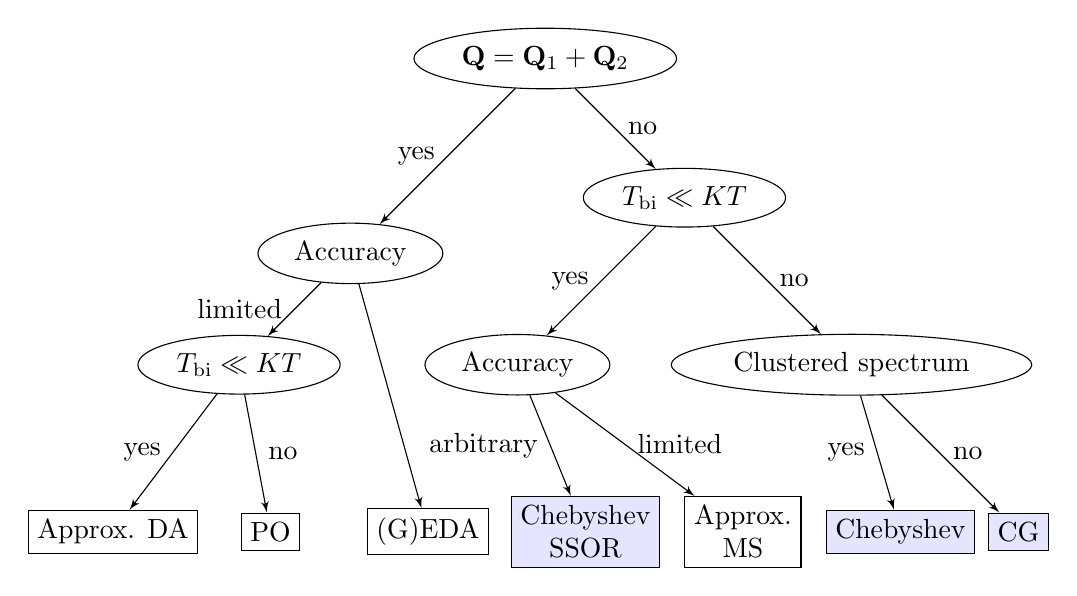
\begin{tikzpicture}[node distance=0.5cm, align=center]

\node (node0) [ellipse,draw=black] {$\B{Q} = \B{Q}_1 + \B{Q}_2$};

\node (node00) [ellipse,draw=black,below left of=node0, node distance=3.5cm] {Accuracy};
\path [line] (node0) -- node [midway,align=center,left=0.1em] {yes} (node00);

\node (node01) [ellipse,draw=black,below right of=node0, node distance=2.5cm] {$T_{\text{bi}} \ll K T$};
\path [line] (node0) -- node [midway,align=center,right=0.1em] {no} (node01);

\node (node010) [ellipse,draw=black,below left of=node01, node distance=3cm] {Accuracy};
\path [line] (node01) -- node [midway,align=center,left=0.1em] {yes} (node010);

\node (node011) [ellipse,draw=black,below right of=node01, node distance=3cm] {Clustered spectrum};
\path [line] (node01) -- node [midway,align=center,right=0.1em] {no} (node011);

\node (node0111) [rectangle,fill=blue!10,draw=black,below right of=node011, node distance=3cm] {CG};
\path [line] (node011) -- node [midway,align=center,right=0.1em] {no} (node0111);

\node (node0110) [rectangle,fill=blue!10,draw=black,left of=node0111, node distance=1.5cm] {Chebyshev};
\path [line] (node011) -- node [midway,align=center,left=0.1em] {yes} (node0110);

\node (node0101) [rectangle,draw=black,left of=node0110, node distance=2cm] {Approx. \\ MS};
\path [line] (node010) -- node [midway,align=center,right=0.1em] {limited} (node0101);

\node (node0100) [rectangle,fill=blue!10,draw=black,left of=node0101, node distance=2cm] {Chebyshev \\ SSOR};
\path [line] (node010) -- node [midway,align=center,left=0.1em] {arbitrary} (node0100);

\node (node000) [rectangle,draw=black,left of=node0100, node distance=2cm] {(G)EDA};
\path [line] (node00) -- node [midway,align=center,right=0.1em] {} (node000);

\node (node001) [ellipse,draw=black,below left of=node00, node distance=2cm] {$T_{\text{bi}} \ll K T$};
\path [line] (node00) -- node [midway,align=center,left=0.1em] {limited} (node001);

\node (node0011) [rectangle,draw=black,left of=node000, node distance=2cm] {PO};
\path [line] (node001) -- node [midway,align=center,right=0.1em] {no} (node0011);

\node (node0010) [rectangle,draw=black,left of=node0011, node distance=2cm] {Approx. DA};
\path [line] (node001) -- node [midway,align=center,left=0.1em] {yes} (node0010);


\end{tikzpicture}
\end{frame}

\subsection{Example}
\begin{frame}
\frametitle{Bayesian Ridge Regression}
Conditional prior for $\Bs{\theta}$: Gaussian i.i.d.,
\[
\begin{aligned}
p(\Bs{\theta}\mid\tau) &\propto \exp\pr{-\frac{1}{2\tau}||\Bs{\theta}||^2},\\
p(\tau) &\propto \dfrac{1}{\tau}\Bs{1}_{\mathbb{R}_+\setminus\{0\}}(\tau).
\end{aligned}
\]
Posterior: 
\[
  \begin{aligned}
    p(\Bs{\theta},\tau \mid \B{y}) \propto \dfrac{1}{\tau}\Bs{1}_{\mathbb{R}_+\setminus\{0\}}(\tau) \ \exp\Big(-\frac{1}{2\tau}||\Bs{\theta}||^2 - \frac{1}{2\sigma^2}||\B{y}-\B{X}\Bs{\theta}||^2\Big).
  \end{aligned}
\]
\end{frame}

\begin{frame}
\frametitle{Bayesian Ridge Regression (Cont.d)}
Conditional posterior distribution associated to $\Bs{\theta}$: Gaussian with precision matrix and mean vector
\[
  \begin{aligned}
    &\B{Q} = \frac{1}{\sigma^{2}}\B{X}^{\top}\B{X} + \tau^{-1}\B{I}_d, \\
    &\Bs{\mu} = \frac{1}{\sigma^{2}} \B{Q}^{-1}\B{X}^{\top}\B{y}. 
  \end{aligned} 
\]
\begin{figure}
    \centering
    \mbox{{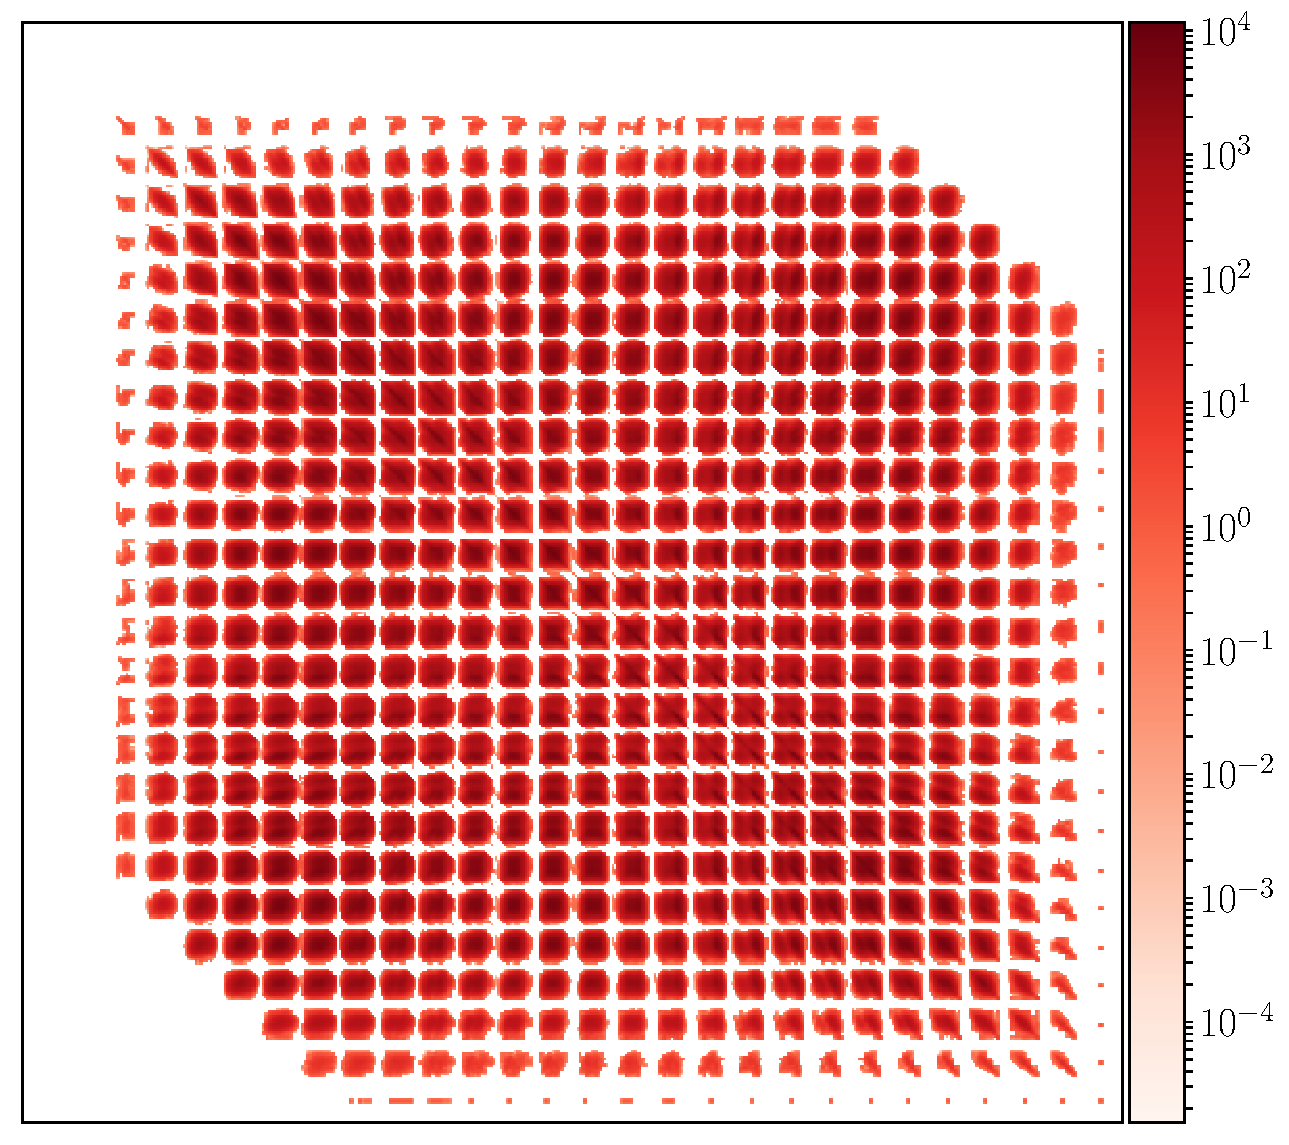
\includegraphics[scale=0.15]{src/images/MNIST_AA.pdf}}}
    \mbox{{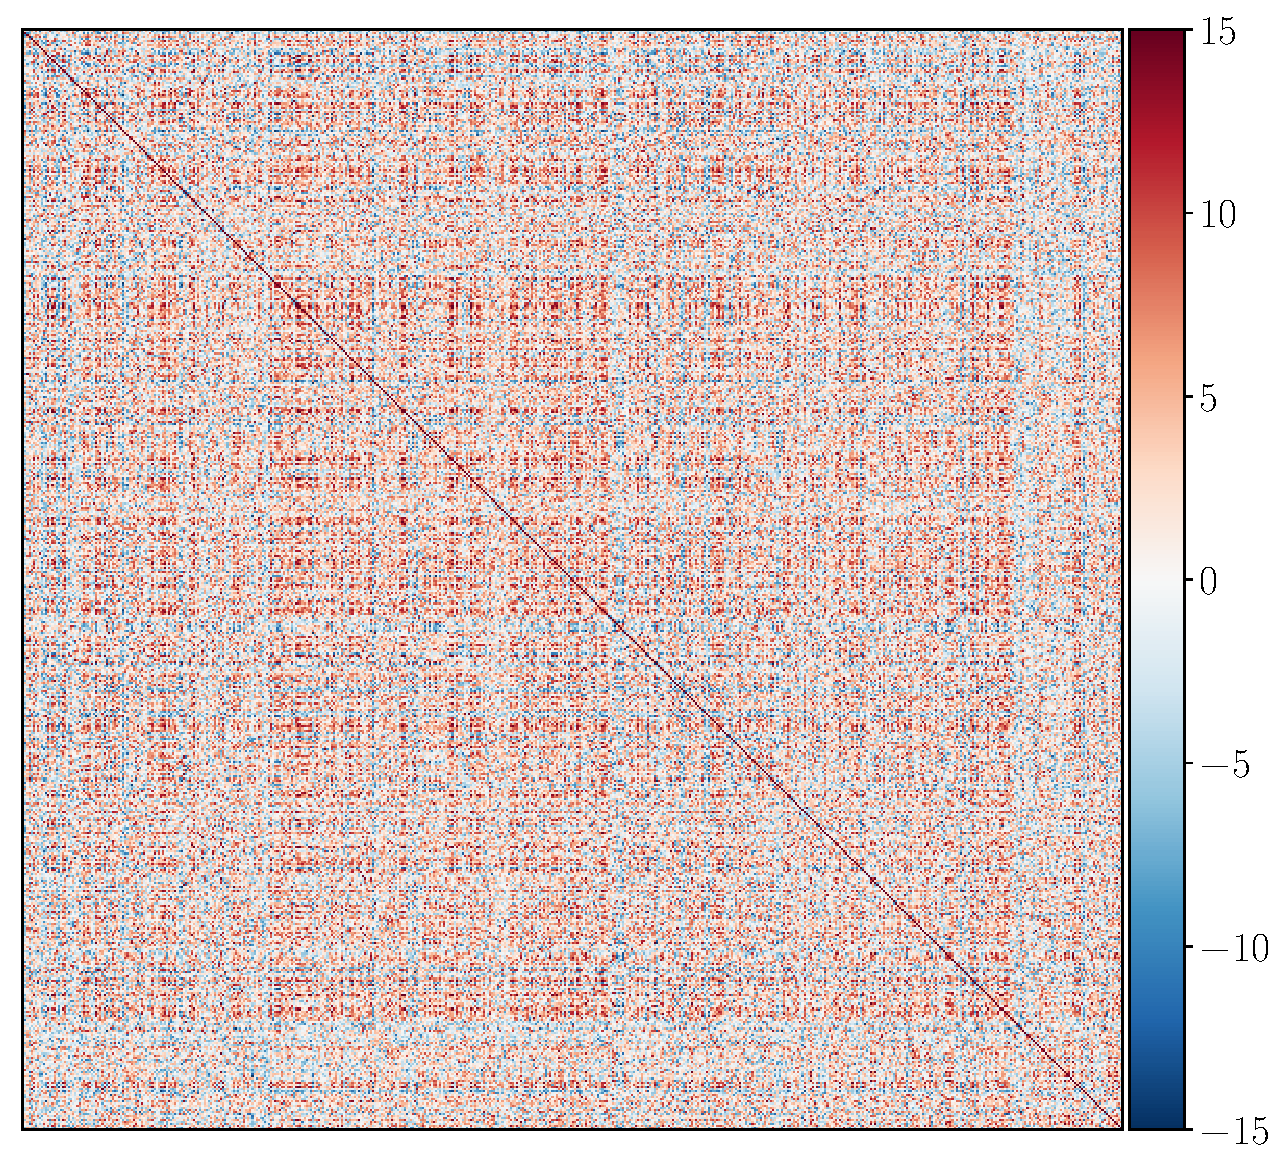
\includegraphics[scale=0.15]{src/images/Armstrong_AA.pdf}}}
    \mbox{{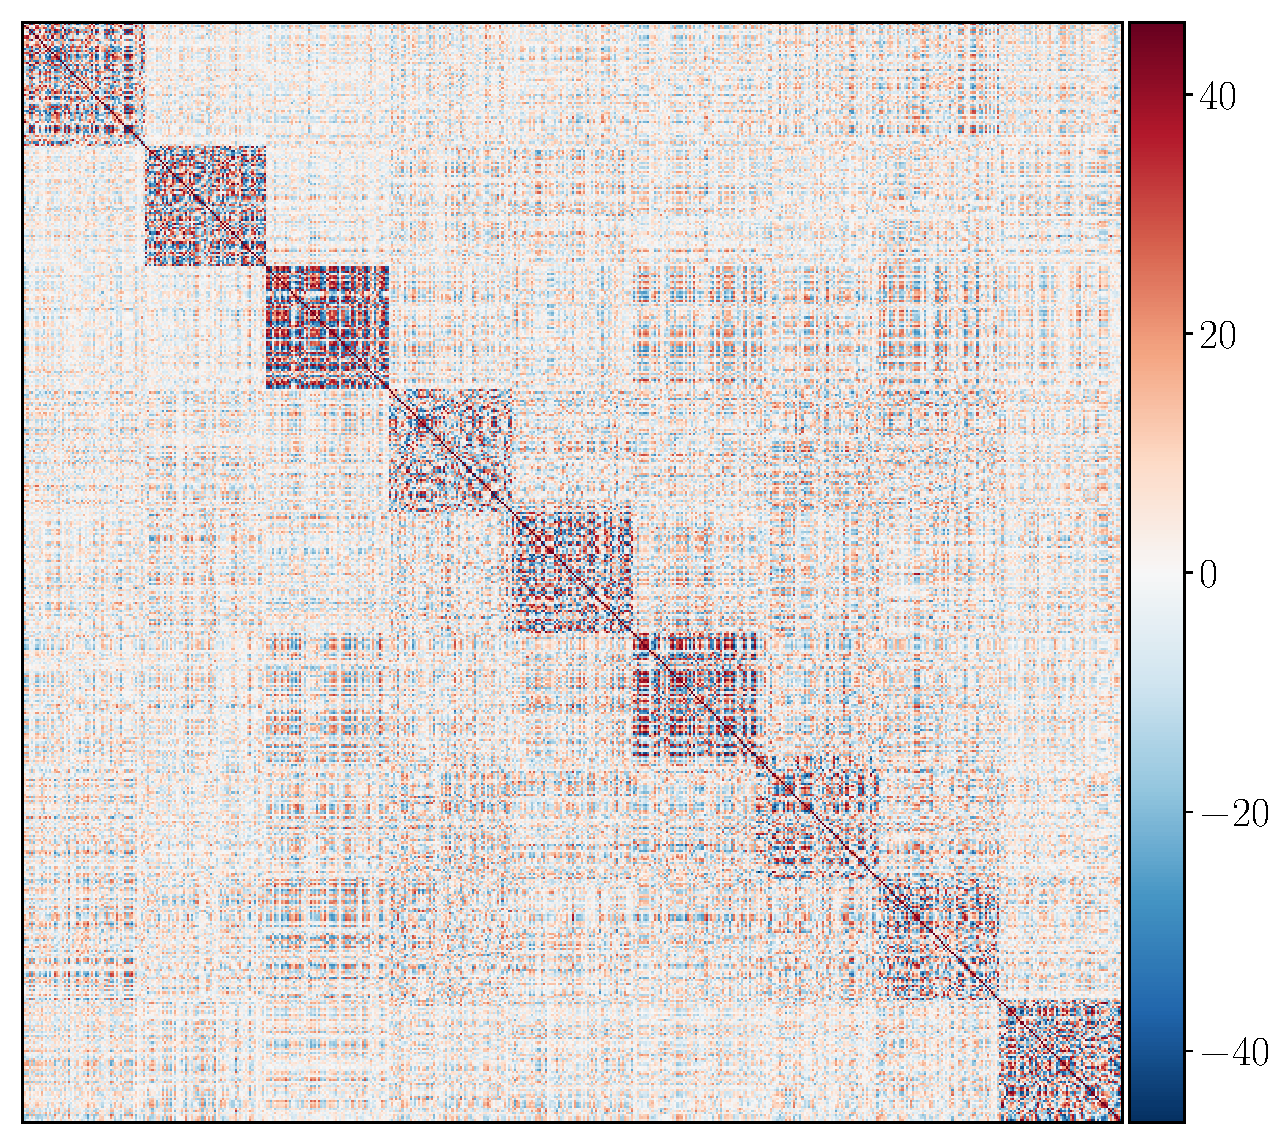
\includegraphics[scale=0.15]{src/images/Coepra_AA.pdf}}}
    \caption{Examples of precision matrices $\B{X}^{\top}\B{X}$ for the MNIST, leukemia abd CoEPrA datasets.}
    \label{fig:LASSO_example}
\end{figure}
\end{frame}

\section{Sampling Algorithms Derived From Numerical Algebra}
\subsection{Polynomial Approximation}
\begin{frame}
\frametitle{Square Root Factorization}
Extension of Cholesky sampler:
\begin{enumerate}
    \item $\B{Q} = \B{U}\B{\Lambda}\B{U^{\top}}$. 
    \item $\B{Q} = \B{B}^2$ with $\B{B} = \B{U}\B{\Lambda}^{1/2}\B{U^{\top}}$.\item $\B{z} \sim \mathcal{N}(\B{0}_d,\B{I}_d)$.
    \item Solve $\B{B}\B{w} = \B{z}$ w.r.t. $\B{w}$ and compute $\Bs{\theta} = \Bs{\mu} + \B{w}$.
\end{enumerate}
We have $f(\B{Q}) = \B{U}f(\B{\Lambda})\B{U}^{\top}$ for real continuous \(f\).

Approximate \(f(\lambda_i) \approx 1/\sqrt{\lambda_i}, \quad \forall i \in [d]\) with Chebyshev polynomials.
\end{frame}

\begin{frame}
\frametitle{Chebyshev Sampler}
The change of interval:
\[g_j = \br{\cos\pr{\pi\frac{2j+1}{2K_{\text{cheby}}}}\dfrac{(\lambda_u-\lambda_l)}{2} + \dfrac{\lambda_u+\lambda_l}{2}}^{-1/2}, \quad j \in [0,K_{\text{cheby}}].\]
The Chebyshev coefficients:
\[c_k = \dfrac{2}{K_{\text{cheby}}} \displaystyle \sum_{j=0}^{K_{\text{cheby}}} g_j \cos\pr{\pi k\frac{2j+1}{2K_{\text{cheby}}}}, \quad k \in [0,K_{\text{cheby}}]. \]
\end{frame}

\begin{frame}
\frametitle{Chebyshev Sampler}
\begin{algorithm}[H]
\caption{Approx.\ square root sampler using Chebyshev polynomials}
\begin{algorithmic}[1] 
\State Draw $\B{z} \sim \mathcal{N}(\B{0}_d,\B{I}_d)$.
\State Set $\alpha = \dfrac{2}{\lambda_u-\lambda_l}$ and $\beta = \dfrac{\lambda_u+\lambda_l}{\lambda_u-\lambda_l}$.
\State Initialize $\B{u}_1 = \alpha\B{Q z} - \beta\B{z}$ and $\B{u}_0 = \B{z}$. 
\State Set $\B{u} = \dfrac{1}{2}c_0\B{u}_0 + c_1\B{u}_1$ and $k=2$.
\While{$k \leq K_{\text{cheby}}$} \Comment{\textcolor{blue}{Compute the $K_{\text{cheby}}$-truncated Chebyshev series.}}
\State Compute $\B{u}' = 2(\alpha\B{Q}\B{u}_1 - \beta\B{u}_1) - \B{u}_0$.
\State Set $\B{u} = \B{u} + c_k\B{u}'$.
\State Set $\B{u}_0 = \B{u}_1$ and $\B{u}_1 = \B{u}'$.
\State $k = k + 1$.
\EndWhile    
\end{algorithmic}
\end{algorithm}
\end{frame}

\subsection{Conjugate Gradient-Based Samplers}
\begin{frame}
\frametitle{Perturbation before Optimization}
Rewrite in \textit{information form}:
\[
  \pi(\Bs{\theta}) \propto \exp\pr{-\dfrac{1}{2}\Bs{\theta}^{\top}\B{Q}\Bs{\theta} + \B{b}^{\top}\Bs{\theta}},
\]
where $\B{b} = \B{Q}\Bs{\mu}$.
\begin{enumerate}
    \item Draw a Gaussian vector $\B{z}' \sim \mathcal{N}(\B{0}_d,\B{Q})$.
    \item Solve a linear system \(\B{Q}\Bs{\theta} = \B{Q}\Bs{\mu} + \B{z}'\) using conjugate gradient methods. (If $\B{u} \sim \mathcal{N}(\B{Q}\Bs{\mu},\B{Q})$, then $\B{Q}^{-1}\B{u} \sim \mathcal{N}(\Bs{\mu},\B{Q}^{-1})$.)
\end{enumerate}
\end{frame}

\begin{frame}
\frametitle{Optimization with Perturbation}
The linear system we solved
\[\B{Q}\Bs{\theta} = \B{b} + \B{z}'\]
can also be seen as a perturbed version of the linear system
\[\B{Q}\Bs{\theta} = \B{b},\]
where $\B{b} = \B{Q}\Bs{\mu}$.

Add a perturbation step (a univariate Gaussian sampling step) to turn the classical CG solver into a CG sampler.

Sequentially builds a Gaussian vector with a covariance matrix being the best $k$-rank approximation of $\B{Q}^{-1}$ in the Krylov subspace $\mathcal{K}_k(\B{Q},\B{r}^{(0)})$. 
\end{frame}

\begin{frame}
\frametitle{CG Sampler}
\begin{algorithmic}[1]
    \State Set $k=1$, $\B{r}^{(0)} = \B{c} - \B{Q}\Bs{\omega}^{(0)}$, $\B{h}^{(0)} = \B{r}^{(0)}$, $d^{(0)} = \B{h}^{(0)\top}\B{Qh}^{(0)}$ and $\B{y}^{(0)} = \Bs{\omega}^{(0)}$. 
    \While{$\nr{\B{r}^{(k)}} \geq \epsilon$} 
    \State Set $\gamma^{(k-1)} = \dfrac{\B{r}^{(k-1)\top}\B{r}^{(k-1)}}{d^{(k-1)}}$.
    \State Set $\B{r}^{(k)} = \B{r}^{(k-1)} - \gamma^{(k-1)}\B{Qh}^{(k-1)}$.
    \State Set $\eta^{(k)} = -\dfrac{\B{r}^{(k)\top}\B{r}^{(k)}}{\B{r}^{(k-1)T}\B{r}^{(k-1)}}$.
    \State Set $\B{h}^{(k)} = \B{r}^{(k)} - \eta^{(k)}\B{h}^{(k-1)}$.
    \State Set $d^{(k)} = \B{h}^{(k)\top}\B{Qh}^{(k)}$.
    \State Set $\B{y}^{(k)} = \B{y}^{(k-1)} + \dfrac{z}{\sqrt{d^{(k-1)}}}\B{h}^{(k-1)}$ where $z \sim \mathcal{N}(0,1)$. \Comment{\textcolor{blue}{Perturbation}} 
    \State $k = k + 1$.
    \EndWhile
    \State Set $\Bs{\theta} = \Bs{\mu} + \B{y}^{(K_{\text{CG}})}$ where $K_{\text{CG}}$ is the number of CG iterations.\\
\Return $\Bs{\theta}$.
\end{algorithmic}
\end{frame}

\subsection{Summary}
\begin{frame}
\frametitle{Iterative Approaches or Factorization Approaches?}
\begin{itemize}
\item Memory needs of order $\Theta(d^2)$ prohibitive. 
\item If storage not an issue, $K \ll (d+T-1)/T$?
\item Gaussian sampling step embedded within a Gibbs sampler, with a varying covariance or precision matrix: $K \ll d$?
\end{itemize}
\end{frame}

\subsection{Experiments}
\begin{frame}
\frametitle{Settings}
\[
    \B{\Sigma}_{ij} = 2 \exp\pr{-\dfrac{(s_i-s_j)^2}{2a^2}} + \epsilon\delta_{ij}, \quad \forall i,j \in [d]. 
\]
where $\{s_{i}\}_{i\in[d]}$ are evenly spaced scalars on $[-3,3]$, $\epsilon > 0$.

$a = 1.5$ and $\epsilon = 10^{-6}$, small eigenvalues of $\B{\Sigma}$ clustered together near $10^{-6}$.

\begin{figure}
\centering
\mbox{{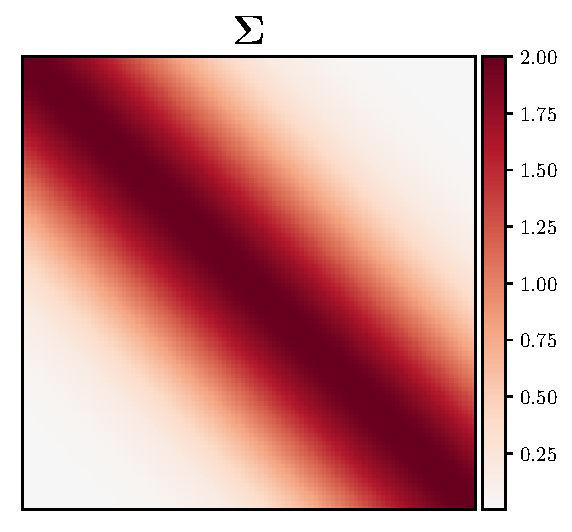
\includegraphics[scale=0.45]{src/images/simu1_ex1_A.pdf}}}
\mbox{{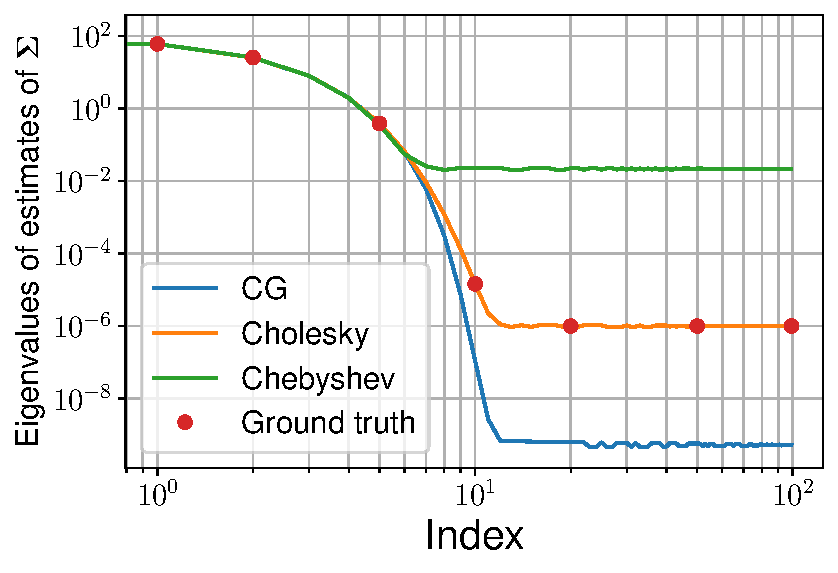
\includegraphics[scale=0.4]{src/images/simu1_ex1_eigvals.pdf}}}
\end{figure}
\end{frame}

\begin{frame}
\frametitle{Results for Accuracy}
\begin{figure}
    \centering
    \mbox{{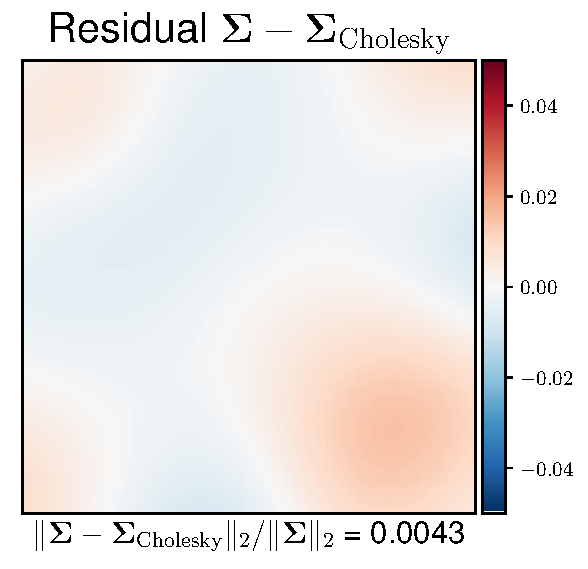
\includegraphics[scale=0.4]{src/images/simu1_ex1_A_Chol.pdf}}}
    \mbox{{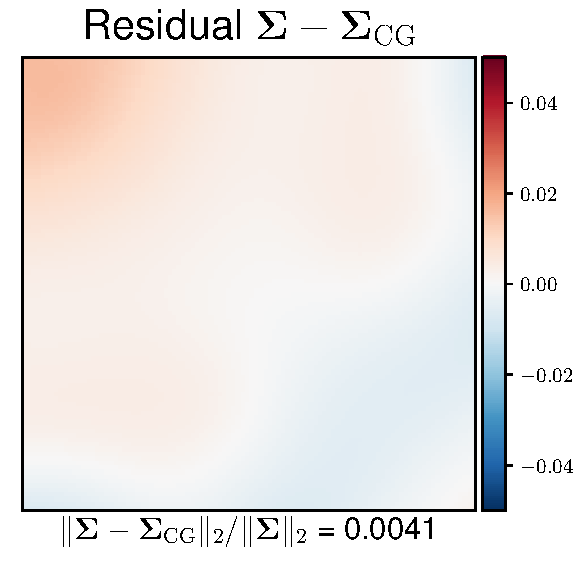
\includegraphics[scale=0.4]{src/images/simu1_ex1_A_CG.pdf}}}
    \mbox{{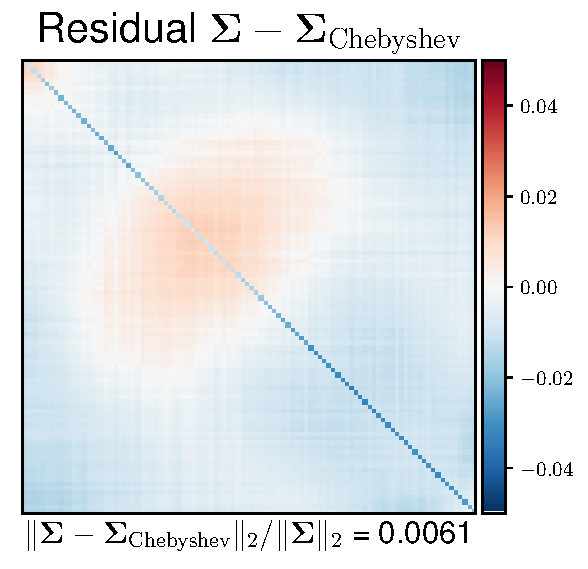
\includegraphics[scale=0.4]{src/images/simu1_ex1_A_Cheby.pdf}}}
  \caption{Scenario 1. Results of the three considered samplers for the sampling from $\mathcal{N}(\B{0}_d,\B{\Sigma})$ in dimension $d = 100$.}
  \end{figure}
\end{frame}

\begin{frame}
\frametitle{Results for CPU Time}
\begin{figure}
    \centering
    \mbox{{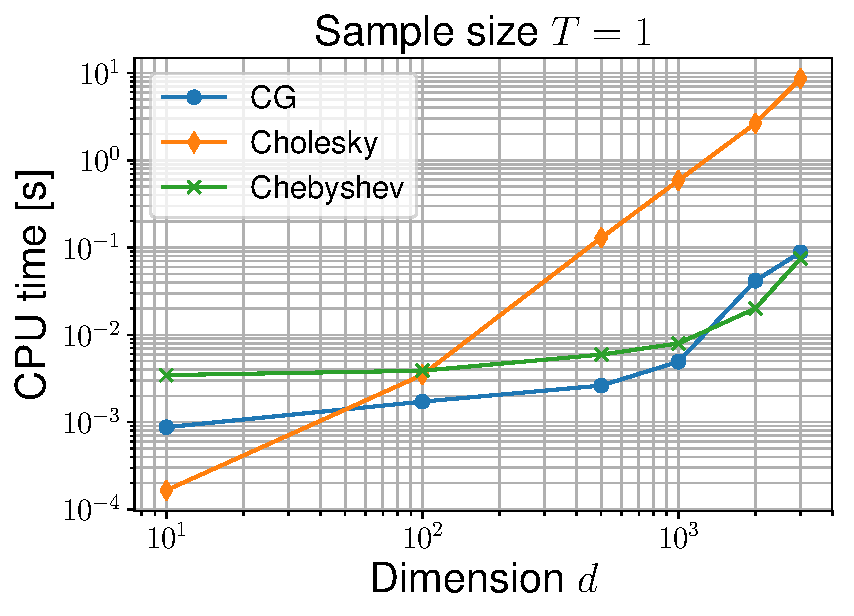
\includegraphics[scale=0.33]{src/images/simu1_ex1_time_1.pdf}}}
    \mbox{{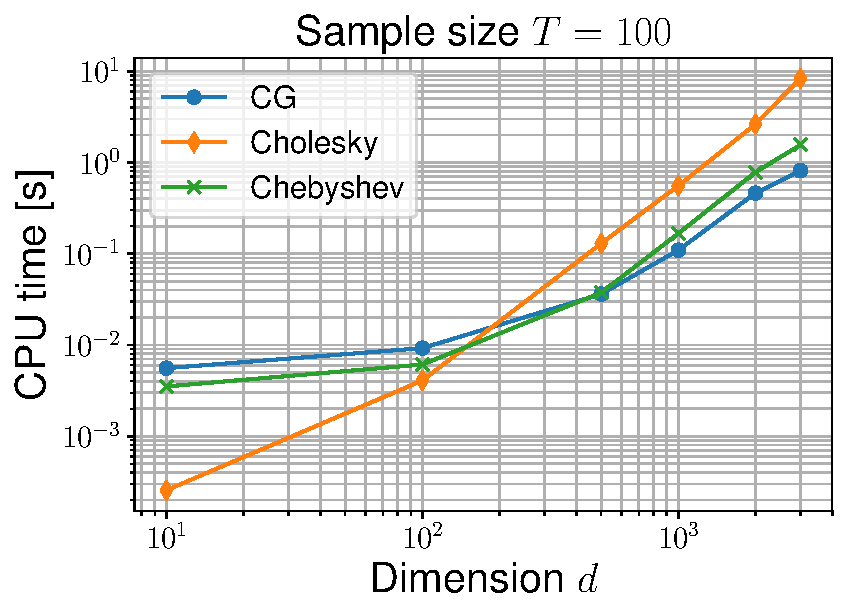
\includegraphics[scale=0.33]{src/images/simu1_ex1_time_100.pdf}}}
    \mbox{{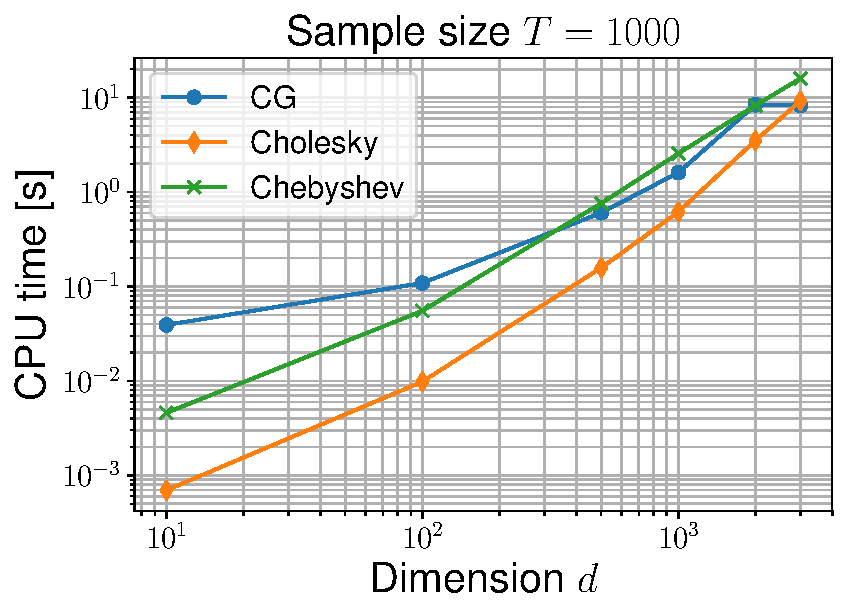
\includegraphics[scale=0.33]{src/images/simu1_ex1_time_1000.pdf}}}
    \mbox{{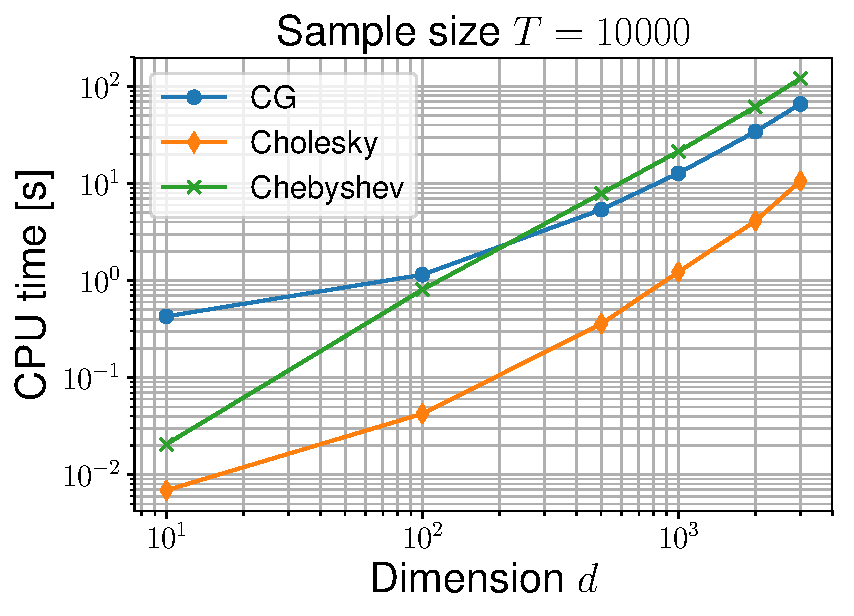
\includegraphics[scale=0.33]{src/images/simu1_ex1_time_10000.pdf}}}
  \end{figure}
\end{frame}

\begin{frame}
\frametitle{Results When Large Eigenvalues Are Clustered}
\begin{figure}
    \centering
    \mbox{{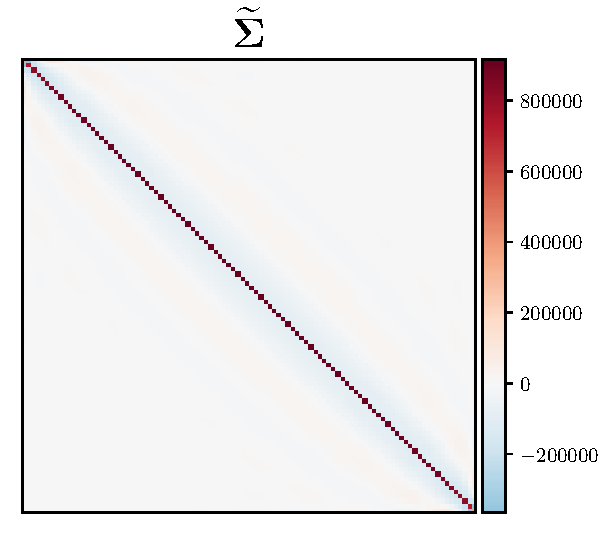
\includegraphics[scale=0.35]{src/images/simu1_ex1_invA.pdf}}}
    \mbox{{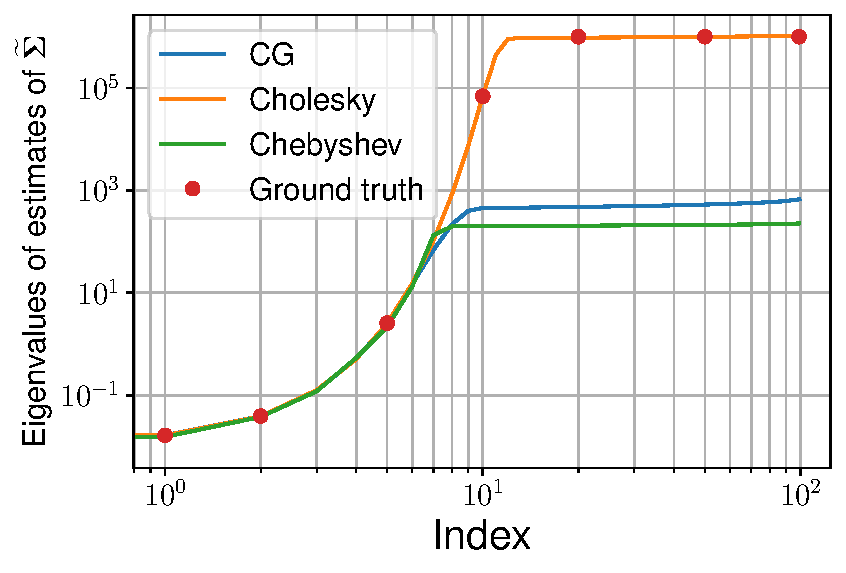
\includegraphics[scale=0.3]{src/images/simu1_ex1_eigvals_invA.pdf}}}
\end{figure}
\begin{figure}
    \centering
    \mbox{{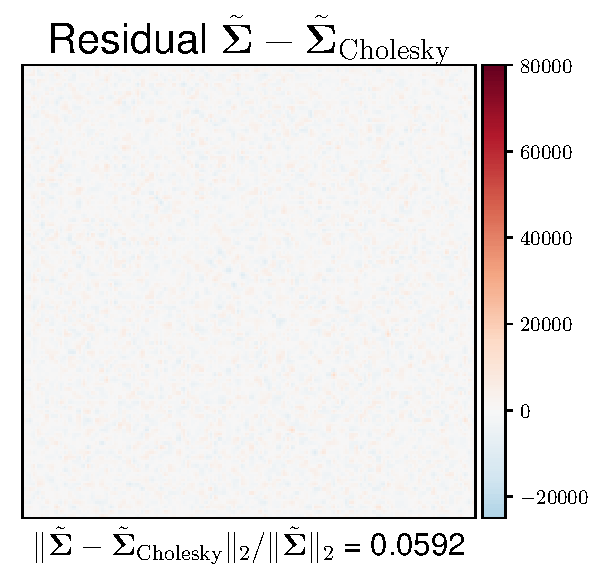
\includegraphics[scale=0.3]{src/images/simu1_ex1_invA_Chol.pdf}}}
    \mbox{{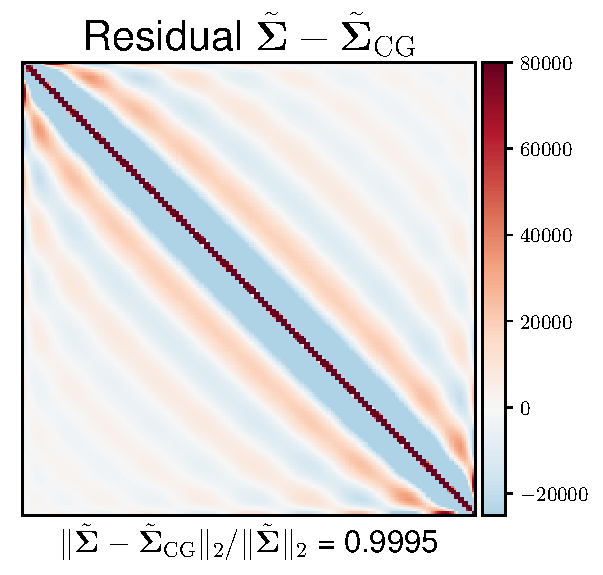
\includegraphics[scale=0.3]{src/images/simu1_ex1_invA_CG.pdf}}}
    \mbox{{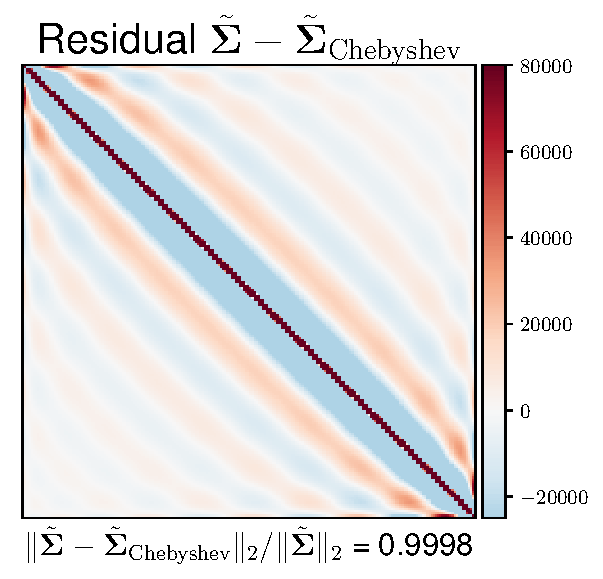
\includegraphics[scale=0.3]{src/images/simu1_ex1_invA_Cheby.pdf}}}
  \end{figure}
\end{frame}

\begin{frame}
\frametitle{CG or Chebyshev?}
\begin{figure}
    \centering
    \mbox{{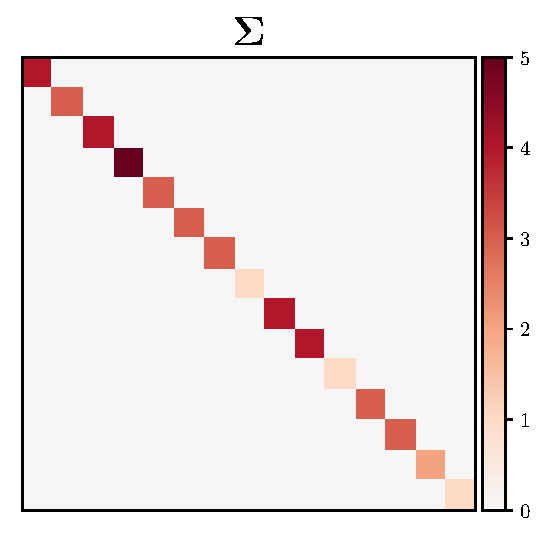
\includegraphics[scale=0.4]{src/images/simu1_ex2_A.pdf}}}
    \mbox{{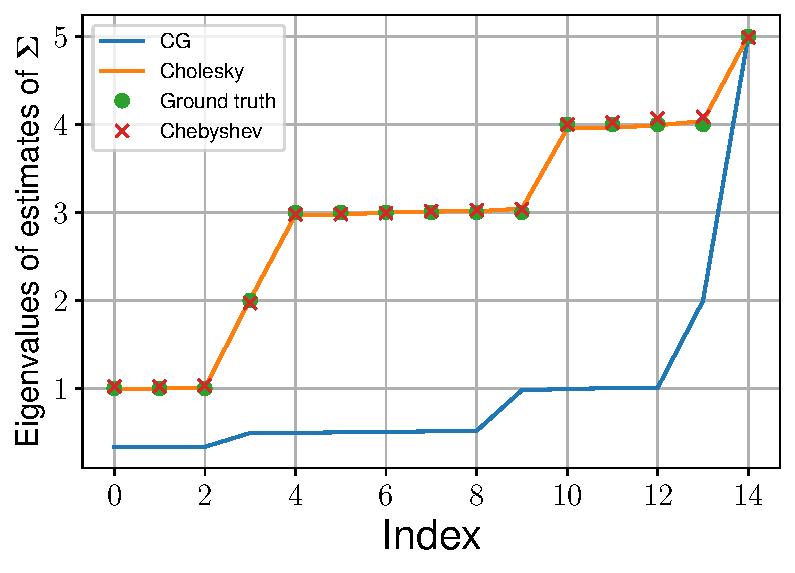
\includegraphics[scale=0.3]{src/images/simu1_ex2_eigvals_A.pdf}}}
\end{figure}
\begin{figure}
    \centering
    \mbox{{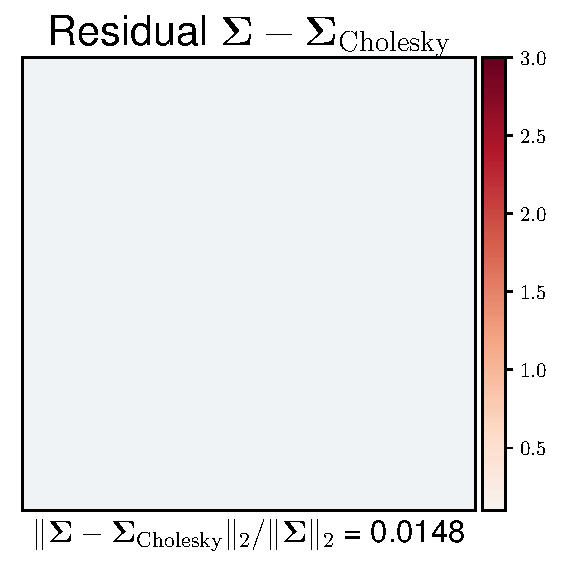
\includegraphics[scale=0.3]{src/images/simu1_ex2_A_Chol.pdf}}}
    \mbox{{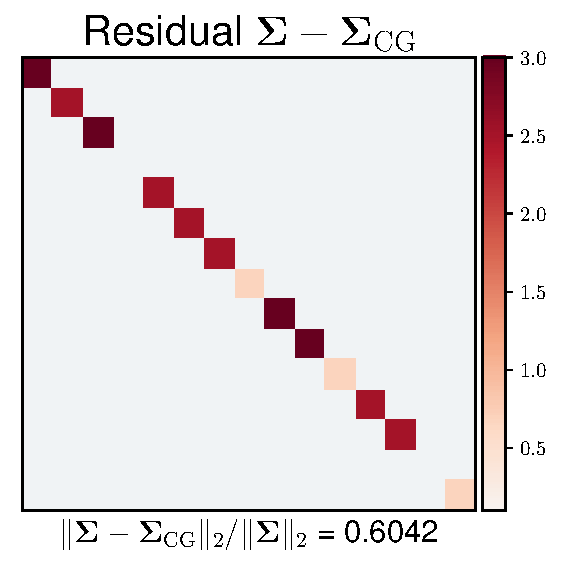
\includegraphics[scale=0.3]{src/images/simu1_ex2_A_CG.pdf}}}
    \mbox{{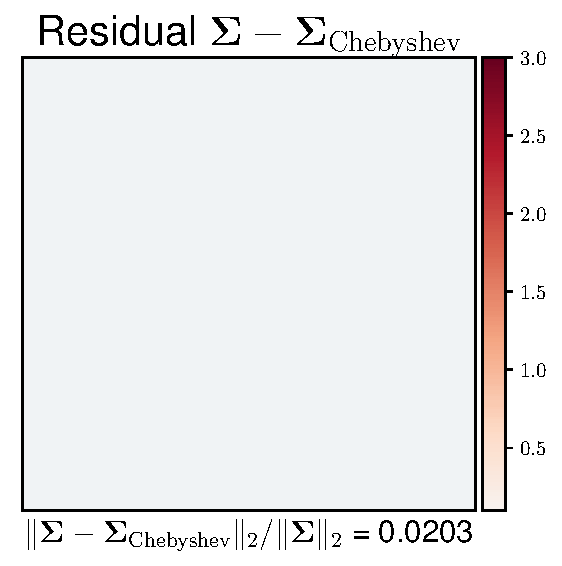
\includegraphics[scale=0.3]{src/images/simu1_ex2_A_Cheby.pdf}}}
  \end{figure}
\end{frame}

\section{Sampling Algorithms Based On MCMC}
\subsection{Matrix Splitting}
\begin{frame}
\frametitle{Conditional Gaussian Distribution}
If $\Bs{\theta} \sim \mathcal{N}(\Bs{\mu},\B{Q}^{-1})$, then
\[
\begin{aligned}
\text{E}(\Bs{\theta}_i | \Bs{\theta}_{-i}) &= \Bs{\mu} - \frac{1}{\B{Q}_{ii} }\sum_{j\ne i} \B{Q}_{ij} (\Bs{\theta}_j - \Bs{\mu}_j), \\
\text{Prec}(\Bs{\theta}_i | \Bs{\theta}_{-i}) &= \B{Q}_{ii}, \\
\text{Corr}(\Bs{\theta}_i, \Bs{\theta}_j | \Bs{\theta}_{-ij}) &= -\frac{\B{Q}_{ij}}{\sqrt{\B{Q}_{ii}\B{Q}_{jj}}}.
\end{aligned}
\]
Compare the above results with
\[
\begin{aligned}
\text{Var}(\Bs{\theta}_i) &= \Bs{\Sigma}_{ii}, \\
\text{Corr}(\Bs{\theta}_i, \Bs{\theta}_j) &= \frac{\Bs{\Sigma}_{ij}}{\sqrt{\Bs{\Sigma}_{ii}\Bs{\Sigma}_{jj}}}.
\end{aligned}
\]
\end{frame}

\begin{frame}
\frametitle{Gibbs Sampler}
\begin{algorithm}[H]
\caption{Component-wise Gibbs sampler}
\hspace*{\algorithmicindent} \textbf{Input:} Number $T$ of iterations and initialization $\Bs{\theta}^{(0)}$.
\begin{algorithmic}[1]
\State Set $t = 1$.
\While{$t\leq T$}
    \For{$i \in [d]$}
    \State Draw $z \sim \mathcal{N}(0,1)$.
    \State Set $\theta^{(t)}_i = \dfrac{[\B{Q}\Bs{\mu}]_i}{Q_{ii}} + \dfrac{z}{\sqrt{Q_{ii}}} - \dfrac{1}{Q_{ii}}\pr{\displaystyle\sum_{j > i}Q_{ij}\theta_j^{(t-1)} + \displaystyle\sum_{j < i}Q_{ij}\theta_j^{(t)}}$.
    \EndFor
    \State Set $t = t + 1$.
\EndWhile\\
\Return $\Bs{\theta}^{(T)}$.
\end{algorithmic}
\end{algorithm}
\end{frame}

\begin{frame}
\frametitle{Rewrite into Gauss--Seidel Linear Systems}
Each iteration solves the linear system
\[(\B{L} + \B{D})\Bs{\theta}^{(t)} = \B{Q}\Bs{\mu} + \B{D}^{1/2}\B{z} - \B{L}^{\top}\Bs{\theta}^{(t-1)},\]
where $\B{z} \sim \mathcal{N}(\B{0}_d,\B{I}_d)$.

By setting $\B{M} = \B{L}+\B{D}$ and $\B{N} = -\B{L}^{\top}$ so that $\B{Q} = \B{M} - \B{N}$,
\[
  \B{M}\Bs{\theta}^{(t)} = \B{Q}\Bs{\mu} +  \tilde{\B{z}}+\B{N}\Bs{\theta}^{(t-1)},
\]
where $\B{N} = -\B{L}^{\top}$ is strictly upper triangular and $\tilde{\B{z}} \sim \mathcal{N}(\B{0}_d,\B{D})$ is easy to sample.
\end{frame}

\begin{frame}
\frametitle{Matrix Splitting Sampler}
\begin{algorithm}[H]
\caption{MCMC sampler based on exact matrix splitting}
\hspace*{\algorithmicindent} \textbf{Input:} Number $T$ of iterations, initialization $\Bs{\theta}^{(0)}$ and splitting $\B{Q} = \B{M} - \B{N}$.
\begin{algorithmic}[1]
\State Set $t=1$.
\While{$t\leq T$}
    \State Draw $\tilde{\B{z}} \sim \mathcal{N}(\B{0}_d,\B{M}^{\top} + \B{N})$.
    \State Solve $\B{M}\Bs{\theta}^{(t)} = \B{Q}\Bs{\mu} + \tilde{\B{z}} + \B{N}\Bs{\theta}^{(t-1)} $ w.r.t. $\Bs{\theta}^{(t)}$.
    \State Set $t = t + 1$.
\EndWhile\\
\Return $\Bs{\theta}^{(T)}$.
\end{algorithmic}
\end{algorithm}
\end{frame}

\begin{frame}
\frametitle{Other Matrix Splitting Schemes}
\begin{table}
{\footnotesize
\caption{The matrices $\B{D}$ and $\B{L}$ denote the diagonal and strictly lower triangular parts of $\B{Q}$, respectively, and $\omega$ is a positive scalar.}
\begin{center}
{\renewcommand{\arraystretch}{1.5}
\begin{tabular}{|l|c|c|c|c|} 
    \hline
    \textbf{Sampler} & $\B{M}$ & $\B{N}$ & $\text{cov}(\tilde{\B{z}}) = \B{M}^{\top} + \B{N}$ & convergence\\
    \hline 
    Richardson & $\B{I}_d/\omega$ & $\B{I}_d/\omega - \B{Q}$ & $2\B{I}_d/\omega - \B{Q}$ & $0 < \omega < 2/\nr{\B{Q}}$\\ 
    Jacobi & $\B{D}$ & $\B{D} - \B{Q}$ & $2\B{D} - \B{Q}$ & $|Q_{ii}| > \sum_{j\neq i}|Q_{ij}|$ $\forall i \in [d]$\\
    Gauss--Seidel & $\B{D} + \B{L}$ & $-\B{L}^{\top}$ & $\B{D}$ & always\\
    SOR & $\B{D}/\omega + \B{L}$ & $\frac{1-\omega}{\omega}\B{D} - \B{L}^{\top}$ & $\frac{2-\omega}{\omega}\B{D}$ & $0 < \omega < 2$\\[1em]
    \hline
\end{tabular}}
\end{center}
}
\end{table}
\end{frame}

\begin{frame}
\frametitle{Error of $t$-th Order Polynomial}
Given a linear system $\B{Q}\Bs{\theta} = \B{v}$ and linear solvers based on the matrix splitting $\B{Q} = \B{M}-\B{N}$, consider the recursion,
\[\Bs{\theta}^{(t+1)} = \Bs{\theta}^{(t)} +  \B{M}^{-1}(\B{v}-\B{Q}\Bs{\theta}^{(t)}).\]

The error at iteration $t$,
\[\B{e}^{(t+1)} = \Bs{\theta}^{(t+1)} - \B{Q}^{-1}\B{v},\]
is equal to 
\[(\B{I}_d-\B{M}^{-1}\B{Q})^t\B{e}^{(0)}.\]

Can we find another $t$-th order polynomial $\mathsf{P}_t$ that achieves a lower error?
\[\rho(\mathsf{P}_t(\B{M}^{-1}\B{Q})) < \rho((\B{I}_d-\B{M}^{-1}\B{Q})^t).\]
\end{frame}

\begin{frame}
\frametitle{Polynomial Accelerated Solver}
Consider the second-order iterative scheme, for any $t \in \mathbb{N}$, 
$$
\Bs{\theta}^{(t+1)} = \alpha_t\Bs{\theta}^{(t)} + (1-\alpha_t)\Bs{\theta}^{(t-1)} + \beta_t \B{M}^{-1}(\B{v}-\B{Q}\Bs{\theta}^{(t)}),
$$
where $(\alpha_t,\beta_t)_{t \in \mathbb{N}}$ are a set of acceleration parameters.

This iterative method yields an error at step $t$ given by 
\[\B{e}^{(t+1)}=\mathsf{P}_t(\B{M}^{-1}\B{Q})\B{e}^{(0)}, \]
where $\mathsf{P}_t$ stands for a scaled Chebyshev polynomial.

Optimal values for $(\alpha_t,\beta_t)_{t \in \mathbb{N}}$ are given by
$$
\alpha_t = \tau_1\beta_t  \quad \text{and} \quad \beta_t = \pr{\tau_1 - \tau_2^2\beta_{t-1}}^{-1} \ , 
$$
$\tau_1 = [\lambda_{\text{min}}(\B{M}^{-1}\B{Q}) + \lambda_{\text{max}}(\B{M}^{-1}\B{Q})]/2$ and $\tau_2 = [\lambda_{\text{max}}(\B{M}^{-1}\B{Q}) - \lambda_{\text{min}}(\B{M}^{-1}\B{Q})]/4$.
\end{frame}

\begin{frame}
\frametitle{Symmetric Splitting Scheme}
Denote by $\B{M}_{\text{SOR}}$ and $\B{N}_{\text{SOR}}$ the matrices involved in the SOR splitting such that $\B{Q} = \B{M}_{\text{SOR}} - \B{N}_{\text{SOR}}$.

Then for any $0<\omega<2$, the SSOR (symmetric SOR) splitting is defined by $\B{Q} = \B{M}_{\text{SSOR}} - \B{N}_{\text{SSOR}}$ with 
$$
\B{M}_{\text{SSOR}} = \frac{\omega}{2-\omega}\B{M}_{\text{SOR}}\B{D}^{-1}\B{M}_{\text{SOR}}^{\top} \quad \text{and} \quad \B{N}_{\text{SSOR}} = \frac{\omega}{2-\omega}\B{N}_{\text{SOR}}\B{D}^{-1}\B{N}_{\text{SOR}}^{\top} \ .
$$
\end{frame}

\begin{frame}
\frametitle{Approximate Matrix Splitting}
\begin{algorithm}[H]
\caption{MCMC sampler based on approximate matrix splitting}
\hspace*{\algorithmicindent} \textbf{Input:} Number $T$ of iterations, initialization $\Bs{\theta}^{(0)}$ and splitting $\B{Q} = \B{M} - \B{N}$.
\begin{algorithmic}[1]
\State Set $t = 1$.
\While{$t\leq T$}
    \State Draw $\tilde{\B{z}}' \sim \mathcal{N}(\B{0}_d,\tilde{\B{M}})$.   \Comment{ {\textcolor{blue}{$\tilde{\B{M}}=\B{D}$ or $2\pr{\B{D}+ 2\omega\B{I}_d}$.}}}
    \State Solve $\B{M}\Bs{\theta}^{(t)} = \B{Q}\Bs{\mu} + \tilde{\B{z}}' + \B{N}\Bs{\theta}^{(t-1)}$.
    \State Set $t = t + 1$.
\EndWhile\\
\Return $\Bs{\theta}^{(T)}$.
\end{algorithmic}
\end{algorithm}
\end{frame}

\subsection{Summary}
\section{Data Augmentation}
\begin{frame}
\frametitle{Iterative Sampler or MCMC Sampler?}
\begin{itemize}
\item Iterative Sampler: $K$ iterations to generate one sample. 
\item MCMC Sampler: burn-in period of length $T_{\text{bi}}$.
\item $T + T_{\text{bi}} \ll KT$?
\item MCMC methods when a large number $T\gtrsim T_{\text{bi}}$ of samples is desired. Iterative methods when a small number $T\lesssim T_{\text{bi}}/K$ of samples is desired.
\end{itemize}
\end{frame}

\section{Data Augmentation}
\begin{frame}
\frametitle{1}
\end{frame}

\section{Unifying Approach Based On Stochastic PPA}
\subsection{PPA}
\begin{frame}
\frametitle{1}
\end{frame}

\end{document}